\documentclass[]{book}
\usepackage{lmodern}
\usepackage{amssymb,amsmath}
\usepackage{ifxetex,ifluatex}
\usepackage{fixltx2e} % provides \textsubscript
\ifnum 0\ifxetex 1\fi\ifluatex 1\fi=0 % if pdftex
  \usepackage[T1]{fontenc}
  \usepackage[utf8]{inputenc}
\else % if luatex or xelatex
  \ifxetex
    \usepackage{mathspec}
  \else
    \usepackage{fontspec}
  \fi
  \defaultfontfeatures{Ligatures=TeX,Scale=MatchLowercase}
\fi
% use upquote if available, for straight quotes in verbatim environments
\IfFileExists{upquote.sty}{\usepackage{upquote}}{}
% use microtype if available
\IfFileExists{microtype.sty}{%
\usepackage{microtype}
\UseMicrotypeSet[protrusion]{basicmath} % disable protrusion for tt fonts
}{}
\usepackage[margin=1in]{geometry}
\usepackage{hyperref}
\hypersetup{unicode=true,
            pdftitle={R Reference book},
            pdfauthor={Reto Zihlmann},
            pdfborder={0 0 0},
            breaklinks=true}
\urlstyle{same}  % don't use monospace font for urls
\usepackage{natbib}
\bibliographystyle{apalike}
\usepackage{color}
\usepackage{fancyvrb}
\newcommand{\VerbBar}{|}
\newcommand{\VERB}{\Verb[commandchars=\\\{\}]}
\DefineVerbatimEnvironment{Highlighting}{Verbatim}{commandchars=\\\{\}}
% Add ',fontsize=\small' for more characters per line
\usepackage{framed}
\definecolor{shadecolor}{RGB}{248,248,248}
\newenvironment{Shaded}{\begin{snugshade}}{\end{snugshade}}
\newcommand{\KeywordTok}[1]{\textcolor[rgb]{0.13,0.29,0.53}{\textbf{#1}}}
\newcommand{\DataTypeTok}[1]{\textcolor[rgb]{0.13,0.29,0.53}{#1}}
\newcommand{\DecValTok}[1]{\textcolor[rgb]{0.00,0.00,0.81}{#1}}
\newcommand{\BaseNTok}[1]{\textcolor[rgb]{0.00,0.00,0.81}{#1}}
\newcommand{\FloatTok}[1]{\textcolor[rgb]{0.00,0.00,0.81}{#1}}
\newcommand{\ConstantTok}[1]{\textcolor[rgb]{0.00,0.00,0.00}{#1}}
\newcommand{\CharTok}[1]{\textcolor[rgb]{0.31,0.60,0.02}{#1}}
\newcommand{\SpecialCharTok}[1]{\textcolor[rgb]{0.00,0.00,0.00}{#1}}
\newcommand{\StringTok}[1]{\textcolor[rgb]{0.31,0.60,0.02}{#1}}
\newcommand{\VerbatimStringTok}[1]{\textcolor[rgb]{0.31,0.60,0.02}{#1}}
\newcommand{\SpecialStringTok}[1]{\textcolor[rgb]{0.31,0.60,0.02}{#1}}
\newcommand{\ImportTok}[1]{#1}
\newcommand{\CommentTok}[1]{\textcolor[rgb]{0.56,0.35,0.01}{\textit{#1}}}
\newcommand{\DocumentationTok}[1]{\textcolor[rgb]{0.56,0.35,0.01}{\textbf{\textit{#1}}}}
\newcommand{\AnnotationTok}[1]{\textcolor[rgb]{0.56,0.35,0.01}{\textbf{\textit{#1}}}}
\newcommand{\CommentVarTok}[1]{\textcolor[rgb]{0.56,0.35,0.01}{\textbf{\textit{#1}}}}
\newcommand{\OtherTok}[1]{\textcolor[rgb]{0.56,0.35,0.01}{#1}}
\newcommand{\FunctionTok}[1]{\textcolor[rgb]{0.00,0.00,0.00}{#1}}
\newcommand{\VariableTok}[1]{\textcolor[rgb]{0.00,0.00,0.00}{#1}}
\newcommand{\ControlFlowTok}[1]{\textcolor[rgb]{0.13,0.29,0.53}{\textbf{#1}}}
\newcommand{\OperatorTok}[1]{\textcolor[rgb]{0.81,0.36,0.00}{\textbf{#1}}}
\newcommand{\BuiltInTok}[1]{#1}
\newcommand{\ExtensionTok}[1]{#1}
\newcommand{\PreprocessorTok}[1]{\textcolor[rgb]{0.56,0.35,0.01}{\textit{#1}}}
\newcommand{\AttributeTok}[1]{\textcolor[rgb]{0.77,0.63,0.00}{#1}}
\newcommand{\RegionMarkerTok}[1]{#1}
\newcommand{\InformationTok}[1]{\textcolor[rgb]{0.56,0.35,0.01}{\textbf{\textit{#1}}}}
\newcommand{\WarningTok}[1]{\textcolor[rgb]{0.56,0.35,0.01}{\textbf{\textit{#1}}}}
\newcommand{\AlertTok}[1]{\textcolor[rgb]{0.94,0.16,0.16}{#1}}
\newcommand{\ErrorTok}[1]{\textcolor[rgb]{0.64,0.00,0.00}{\textbf{#1}}}
\newcommand{\NormalTok}[1]{#1}
\usepackage{longtable,booktabs}
\usepackage{graphicx,grffile}
\makeatletter
\def\maxwidth{\ifdim\Gin@nat@width>\linewidth\linewidth\else\Gin@nat@width\fi}
\def\maxheight{\ifdim\Gin@nat@height>\textheight\textheight\else\Gin@nat@height\fi}
\makeatother
% Scale images if necessary, so that they will not overflow the page
% margins by default, and it is still possible to overwrite the defaults
% using explicit options in \includegraphics[width, height, ...]{}
\setkeys{Gin}{width=\maxwidth,height=\maxheight,keepaspectratio}
\IfFileExists{parskip.sty}{%
\usepackage{parskip}
}{% else
\setlength{\parindent}{0pt}
\setlength{\parskip}{6pt plus 2pt minus 1pt}
}
\setlength{\emergencystretch}{3em}  % prevent overfull lines
\providecommand{\tightlist}{%
  \setlength{\itemsep}{0pt}\setlength{\parskip}{0pt}}
\setcounter{secnumdepth}{5}
% Redefines (sub)paragraphs to behave more like sections
\ifx\paragraph\undefined\else
\let\oldparagraph\paragraph
\renewcommand{\paragraph}[1]{\oldparagraph{#1}\mbox{}}
\fi
\ifx\subparagraph\undefined\else
\let\oldsubparagraph\subparagraph
\renewcommand{\subparagraph}[1]{\oldsubparagraph{#1}\mbox{}}
\fi

%%% Use protect on footnotes to avoid problems with footnotes in titles
\let\rmarkdownfootnote\footnote%
\def\footnote{\protect\rmarkdownfootnote}

%%% Change title format to be more compact
\usepackage{titling}

% Create subtitle command for use in maketitle
\newcommand{\subtitle}[1]{
  \posttitle{
    \begin{center}\large#1\end{center}
    }
}

\setlength{\droptitle}{-2em}

  \title{R Reference book}
    \pretitle{\vspace{\droptitle}\centering\huge}
  \posttitle{\par}
    \author{Reto Zihlmann}
    \preauthor{\centering\large\emph}
  \postauthor{\par}
      \predate{\centering\large\emph}
  \postdate{\par}
    \date{2019-04-04}

\usepackage{booktabs}

\begin{document}
\maketitle

{
\setcounter{tocdepth}{1}
\tableofcontents
}
\chapter{Introduction}\label{introduction}

\begin{center}
\includegraphics[width=0.7\linewidth]{figures/01_cover/Cover2} \end{center}

\begin{center}\rule{0.5\linewidth}{\linethickness}\end{center}

This book contains a not final and constantely growing collection of
useful R knowledge. \href{https://www.r-project.org/}{R} is a free
software environment for statistical computing and graphics. The book is
written in \href{https://rmarkdown.rstudio.com/}{RMarkdown} with
\href{https://bookdown.org/}{bookdown}.

\begin{center}\rule{0.5\linewidth}{\linethickness}\end{center}

This work is licensed under a Creative Commons
Attribution-NonCommercial-ShareAlike 4.0 International License.

\begin{center}\rule{0.5\linewidth}{\linethickness}\end{center}

\chapter{Plots}\label{Plots}

\section{\texorpdfstring{Graphical parameters
\texttt{par()}}{Graphical parameters par()}}\label{graphical-parameters-par}

\subsection{Set graphical parameters}\label{set-graphical-parameters}

Change global option

\begin{Shaded}
\begin{Highlighting}[]
\KeywordTok{par}\NormalTok{(}\DataTypeTok{xlog =}\NormalTok{ T)}
\end{Highlighting}
\end{Shaded}

change for local plot

\begin{Shaded}
\begin{Highlighting}[]
\KeywordTok{plot}\NormalTok{(..., }\DataTypeTok{xlog =}\NormalTok{ T)}
\end{Highlighting}
\end{Shaded}

When parameters are set, their previous values are returned in an
invisible named list. Such a list can be passed as an argument to par to
restore the parameter values.

\begin{Shaded}
\begin{Highlighting}[]
\NormalTok{opar <-}\StringTok{ }\KeywordTok{par}\NormalTok{(}\DataTypeTok{xlog =}\NormalTok{ T)}
\KeywordTok{plot}\NormalTok{(...)}
\KeywordTok{par}\NormalTok{(opar)}
\end{Highlighting}
\end{Shaded}

reset default

\begin{Shaded}
\begin{Highlighting}[]
\KeywordTok{dev.off}\NormalTok{()}
\end{Highlighting}
\end{Shaded}

check current parameter

\begin{Shaded}
\begin{Highlighting}[]
\KeywordTok{par}\NormalTok{(}\StringTok{"xlog"}\NormalTok{)}
\end{Highlighting}
\end{Shaded}

\begin{verbatim}
#> [1] FALSE
\end{verbatim}

The parameters are defined for the currently active device

\begin{itemize}
\tightlist
\item
  Normally the Rstudio plot panel
\item
  If \texttt{png()} or \texttt{pdf()} opend =\textgreater{} only within
  this document
\item
  \texttt{dev.off()} closes device and reset \texttt{par()}

  \begin{itemize}
  \tightlist
  \item
    If \texttt{png()} or \texttt{pdf()}   ⇒ the same par are active as
    they were before the device \texttt{png()} or \texttt{pdf()} was
    opend
  \item
    If Rstudio panel \t   ⇒ the default par are active
  \end{itemize}
\end{itemize}

\subsection{Default}\label{default}

\begin{Shaded}
\begin{Highlighting}[]
\KeywordTok{par}\NormalTok{()}
\end{Highlighting}
\end{Shaded}

\begin{verbatim}
#> $xlog
#> [1] FALSE
#> 
#> $ylog
#> [1] FALSE
#> 
#> $adj
#> [1] 0.5
#> 
#> $ann
#> [1] TRUE
#> 
#> $ask
#> [1] FALSE
#> 
#> $bg
#> [1] "transparent"
#> 
#> $bty
#> [1] "o"
#> 
#> $cex
#> [1] 1
#> 
#> $cex.axis
#> [1] 1
#> 
#> $cex.lab
#> [1] 1
#> 
#> $cex.main
#> [1] 1.2
#> 
#> $cex.sub
#> [1] 1
#> 
#> $cin
#> [1] 0.15 0.20
#> 
#> $col
#> [1] "black"
#> 
#> $col.axis
#> [1] "black"
#> 
#> $col.lab
#> [1] "black"
#> 
#> $col.main
#> [1] "black"
#> 
#> $col.sub
#> [1] "black"
#> 
#> $cra
#> [1] 10.8 14.4
#> 
#> $crt
#> [1] 0
#> 
#> $csi
#> [1] 0.2
#> 
#> $cxy
#> [1] 0.02851711 0.07518797
#> 
#> $din
#> [1] 6.5 4.5
#> 
#> $err
#> [1] 0
#> 
#> $family
#> [1] ""
#> 
#> $fg
#> [1] "black"
#> 
#> $fig
#> [1] 0 1 0 1
#> 
#> $fin
#> [1] 6.5 4.5
#> 
#> $font
#> [1] 1
#> 
#> $font.axis
#> [1] 1
#> 
#> $font.lab
#> [1] 1
#> 
#> $font.main
#> [1] 2
#> 
#> $font.sub
#> [1] 1
#> 
#> $lab
#> [1] 5 5 7
#> 
#> $las
#> [1] 0
#> 
#> $lend
#> [1] "round"
#> 
#> $lheight
#> [1] 1
#> 
#> $ljoin
#> [1] "round"
#> 
#> $lmitre
#> [1] 10
#> 
#> $lty
#> [1] "solid"
#> 
#> $lwd
#> [1] 1
#> 
#> $mai
#> [1] 1.02 0.82 0.82 0.42
#> 
#> $mar
#> [1] 5.1 4.1 4.1 2.1
#> 
#> $mex
#> [1] 1
#> 
#> $mfcol
#> [1] 1 1
#> 
#> $mfg
#> [1] 1 1 1 1
#> 
#> $mfrow
#> [1] 1 1
#> 
#> $mgp
#> [1] 3 1 0
#> 
#> $mkh
#> [1] 0.001
#> 
#> $new
#> [1] FALSE
#> 
#> $oma
#> [1] 0 0 0 0
#> 
#> $omd
#> [1] 0 1 0 1
#> 
#> $omi
#> [1] 0 0 0 0
#> 
#> $page
#> [1] TRUE
#> 
#> $pch
#> [1] 1
#> 
#> $pin
#> [1] 5.26 2.66
#> 
#> $plt
#> [1] 0.1261538 0.9353846 0.2266667 0.8177778
#> 
#> $ps
#> [1] 12
#> 
#> $pty
#> [1] "m"
#> 
#> $smo
#> [1] 1
#> 
#> $srt
#> [1] 0
#> 
#> $tck
#> [1] NA
#> 
#> $tcl
#> [1] -0.5
#> 
#> $usr
#> [1] 0 1 0 1
#> 
#> $xaxp
#> [1] 0 1 5
#> 
#> $xaxs
#> [1] "r"
#> 
#> $xaxt
#> [1] "s"
#> 
#> $xpd
#> [1] FALSE
#> 
#> $yaxp
#> [1] 0 1 5
#> 
#> $yaxs
#> [1] "r"
#> 
#> $yaxt
#> [1] "s"
#> 
#> $ylbias
#> [1] 0.2
\end{verbatim}

\subsection{Device region}\label{device-region}

\begin{Shaded}
\begin{Highlighting}[]
\NormalTok{opar <-}\StringTok{ }\KeywordTok{par}\NormalTok{(}\DataTypeTok{xpd =} \OtherTok{NA}\NormalTok{,}
    \DataTypeTok{mar =} \KeywordTok{c}\NormalTok{(}\DecValTok{5}\NormalTok{,}\DecValTok{4}\NormalTok{,}\DecValTok{4}\NormalTok{,}\DecValTok{2}\NormalTok{) }\OperatorTok{+}\StringTok{ }\FloatTok{0.1}\NormalTok{,}
    \DataTypeTok{oma =} \KeywordTok{c}\NormalTok{(}\DecValTok{3}\NormalTok{,}\DecValTok{3}\NormalTok{,}\DecValTok{3}\NormalTok{,}\DecValTok{3}\NormalTok{) }\OperatorTok{+}\StringTok{ }\FloatTok{0.05}\NormalTok{)}

\KeywordTok{plot}\NormalTok{(}\DecValTok{1}\OperatorTok{:}\DecValTok{10}\NormalTok{, }\DecValTok{1}\OperatorTok{:}\DecValTok{10}\NormalTok{, }\DataTypeTok{type =} \StringTok{"n"}\NormalTok{,}
     \DataTypeTok{xlab =} \StringTok{""}\NormalTok{, }\DataTypeTok{ylab =} \StringTok{"Y"}\NormalTok{)}

\KeywordTok{box}\NormalTok{(}\StringTok{"plot"}\NormalTok{, }\DataTypeTok{col =} \StringTok{"red"}\NormalTok{)}
\KeywordTok{box}\NormalTok{(}\StringTok{"inner"}\NormalTok{, }\DataTypeTok{col =} \StringTok{"green"}\NormalTok{)}
\KeywordTok{box}\NormalTok{(}\StringTok{"outer"}\NormalTok{, }\DataTypeTok{col =} \StringTok{"blue"}\NormalTok{)}

\KeywordTok{text}\NormalTok{(}\DecValTok{5}\NormalTok{,}\DecValTok{9}\NormalTok{, }\StringTok{"Plot"}\NormalTok{, }\DataTypeTok{col =} \StringTok{"red"}\NormalTok{, }\DataTypeTok{cex  =} \DecValTok{2}\NormalTok{)}
\KeywordTok{mtext}\NormalTok{(}\StringTok{"Figure"}\NormalTok{, }\DataTypeTok{col =} \StringTok{"green"}\NormalTok{, }\DataTypeTok{cex =} \DecValTok{2}\NormalTok{,}
      \DataTypeTok{side =} \DecValTok{3}\NormalTok{, }\DataTypeTok{line =} \DecValTok{2}\NormalTok{)}
\KeywordTok{mtext}\NormalTok{(}\StringTok{"Device"}\NormalTok{, }\DataTypeTok{col =} \StringTok{"blue"}\NormalTok{, }\DataTypeTok{cex =} \DecValTok{2}\NormalTok{,}
      \DataTypeTok{side =} \DecValTok{3}\NormalTok{, }\DataTypeTok{line =} \DecValTok{1}\NormalTok{, }\DataTypeTok{outer =}\NormalTok{ T)}

\KeywordTok{mtext}\NormalTok{(}\DataTypeTok{text =} \KeywordTok{c}\NormalTok{(}\StringTok{"Line 0"}\NormalTok{,}
               \StringTok{"Line 1"}\NormalTok{,}
               \StringTok{"Line 2"}\NormalTok{,}
               \StringTok{"Line 3"}\NormalTok{),}
      \DataTypeTok{side =} \DecValTok{3}\NormalTok{, }\DataTypeTok{line =} \DecValTok{0}\OperatorTok{:}\DecValTok{3}\NormalTok{,}
      \DataTypeTok{at =} \KeywordTok{grconvertX}\NormalTok{(}\DecValTok{1}\NormalTok{, }\StringTok{"npc"}\NormalTok{, }\StringTok{"user"}\NormalTok{),}
      \DataTypeTok{adj =} \DecValTok{1}\NormalTok{,}
      \DataTypeTok{col =} \StringTok{"green"}\NormalTok{)}

\KeywordTok{mtext}\NormalTok{(}\DataTypeTok{text =} \KeywordTok{c}\NormalTok{(}\StringTok{"Line 0"}\NormalTok{,}
               \StringTok{"Line 1"}\NormalTok{,}
               \StringTok{"Line 2"}\NormalTok{,}
               \StringTok{"Line 3"}\NormalTok{),}
      \DataTypeTok{side =} \DecValTok{2}\NormalTok{, }\DataTypeTok{line =} \DecValTok{0}\OperatorTok{:}\DecValTok{3}\NormalTok{,}
      \DataTypeTok{adj =} \DecValTok{1}\NormalTok{,}
      \DataTypeTok{col =} \StringTok{"green"}\NormalTok{)}

\KeywordTok{mtext}\NormalTok{(}\DataTypeTok{text =} \KeywordTok{c}\NormalTok{(}\StringTok{"Line 0"}\NormalTok{,}
               \StringTok{"Line 1"}\NormalTok{,}
               \StringTok{"Line 2"}\NormalTok{),}
      \DataTypeTok{side =} \DecValTok{1}\NormalTok{, }\DataTypeTok{line =} \DecValTok{0}\OperatorTok{:}\DecValTok{2}\NormalTok{, }\DataTypeTok{outer =}\NormalTok{ T,}
      \DataTypeTok{at =} \DecValTok{0}\NormalTok{, }\DataTypeTok{adj =} \DecValTok{0}\NormalTok{,}
      \DataTypeTok{col =} \StringTok{"blue"}\NormalTok{)}


\KeywordTok{mtext}\NormalTok{(}\DataTypeTok{text =} \StringTok{"Margins"}\NormalTok{,}
      \DataTypeTok{side =} \DecValTok{1}\NormalTok{, }\DataTypeTok{line =} \DecValTok{2}\NormalTok{, }\DataTypeTok{cex =} \DecValTok{2}\NormalTok{)}
\KeywordTok{mtext}\NormalTok{(}\DataTypeTok{text =} \StringTok{"par(mar=c(5,4,4,2) + 0.1)"}\NormalTok{,}
      \DataTypeTok{side =} \DecValTok{1}\NormalTok{, }\DataTypeTok{line =} \DecValTok{3}\NormalTok{)}

\KeywordTok{mtext}\NormalTok{(}\DataTypeTok{text =} \StringTok{"Outer Margin"}\NormalTok{,}
      \DataTypeTok{side =} \DecValTok{1}\NormalTok{, }\DataTypeTok{line =} \DecValTok{1}\NormalTok{, }\DataTypeTok{cex =} \DecValTok{2}\NormalTok{, }\DataTypeTok{outer =}\NormalTok{ T)}
\KeywordTok{mtext}\NormalTok{(}\DataTypeTok{text =} \StringTok{"par(oma=c(3,3,3,3))"}\NormalTok{,}
      \DataTypeTok{side =} \DecValTok{1}\NormalTok{, }\DataTypeTok{line =} \DecValTok{2}\NormalTok{, }\DataTypeTok{outer =}\NormalTok{ T)}
\end{Highlighting}
\end{Shaded}

\begin{center}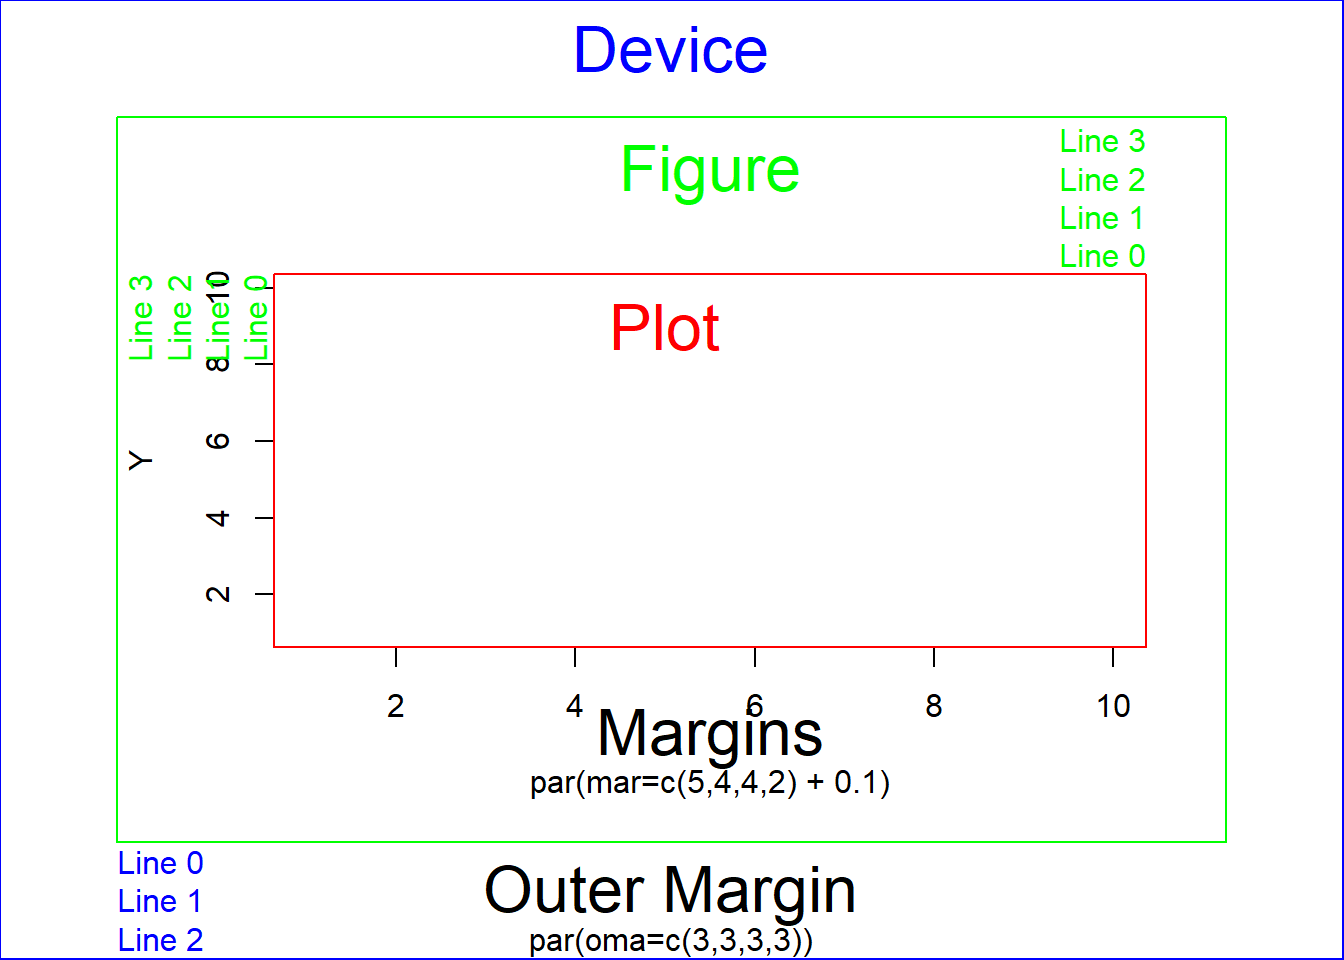
\includegraphics{R_Ref_Book_files/figure-latex/unnamed-chunk-10-1} \end{center}

\begin{Shaded}
\begin{Highlighting}[]
\KeywordTok{par}\NormalTok{(opar)}
\end{Highlighting}
\end{Shaded}

\subsubsection{Coordinate system outside
plot}\label{coordinate-system-outside-plot}

\begin{Shaded}
\begin{Highlighting}[]
\KeywordTok{par}\NormalTok{(}\StringTok{"mar"}\NormalTok{) }\CommentTok{# Margine Area}
\CommentTok{#> [1] 5.1 4.1 4.1 2.1}
\KeywordTok{par}\NormalTok{(}\StringTok{"oma"}\NormalTok{) }\CommentTok{# Outer Margin Area}
\CommentTok{#> [1] 0 0 0 0}
\KeywordTok{par}\NormalTok{(}\StringTok{"mgp"}\NormalTok{) }\CommentTok{# position of [1] x/y-label, [2] axis, [3] ticks}
\CommentTok{#> [1] 3 1 0}
\KeywordTok{par}\NormalTok{(}\StringTok{"mex"}\NormalTok{) }\CommentTok{# "height"" of one line}
\CommentTok{#> [1] 1}
\end{Highlighting}
\end{Shaded}

\subsubsection{Normalized device coordinates (NDC) {[}0,
1{]}}\label{normalized-device-coordinates-ndc-0-1}

\begin{Shaded}
\begin{Highlighting}[]
\KeywordTok{par}\NormalTok{(}\StringTok{"fig"}\NormalTok{) }\CommentTok{# Start and endpoint of ploting region}
\CommentTok{#> [1] 0 1 0 1}
\KeywordTok{par}\NormalTok{(}\StringTok{"omd"}\NormalTok{) }\CommentTok{# oma in NDC}
\CommentTok{#> [1] 0 1 0 1}
\end{Highlighting}
\end{Shaded}

\subsubsection{Change between coordinate
system}\label{change-between-coordinate-system}

Use \texttt{grconvertX()} to change between different coordinate systems

\subsubsection{Plot outside plotting
region}\label{plot-outside-plotting-region}

\begin{Shaded}
\begin{Highlighting}[]
\KeywordTok{par}\NormalTok{(}\StringTok{"xpd"}\NormalTok{)}
\CommentTok{#> [1] FALSE}
\end{Highlighting}
\end{Shaded}

\texttt{FALSE} \(\Rightarrow\) clipped to the plot regions\\
\texttt{TRUE} ⇒ clipped to the figure region\\
\texttt{NA} ⇒ clipped to the device region

\chapter{Methods}\label{methods}

We describe our methods in this chapter.

\chapter{Applications}\label{applications}

Some \emph{significant} applications are demonstrated in this chapter.

\section{Example one}\label{example-one}

\section{Example two}\label{example-two}

\chapter{Final Words}\label{final-words}

\begin{center}\rule{0.5\linewidth}{\linethickness}\end{center}

You can label chapter and section titles using \texttt{\{\#label\}}
after them, e.g., we can reference Chapter \ref{intro}. If you do not
manually label them, there will be automatic labels anyway, e.g.,
Chapter \ref{methods}.

Figures and tables with captions will be placed in \texttt{figure} and
\texttt{table} environments, respectively.

\begin{Shaded}
\begin{Highlighting}[]
\KeywordTok{par}\NormalTok{(}\DataTypeTok{mar =} \KeywordTok{c}\NormalTok{(}\DecValTok{4}\NormalTok{, }\DecValTok{4}\NormalTok{, .}\DecValTok{1}\NormalTok{, .}\DecValTok{1}\NormalTok{))}
\KeywordTok{plot}\NormalTok{(pressure, }\DataTypeTok{type =} \StringTok{'b'}\NormalTok{, }\DataTypeTok{pch =} \DecValTok{19}\NormalTok{)}
\end{Highlighting}
\end{Shaded}

\begin{figure}

{\centering 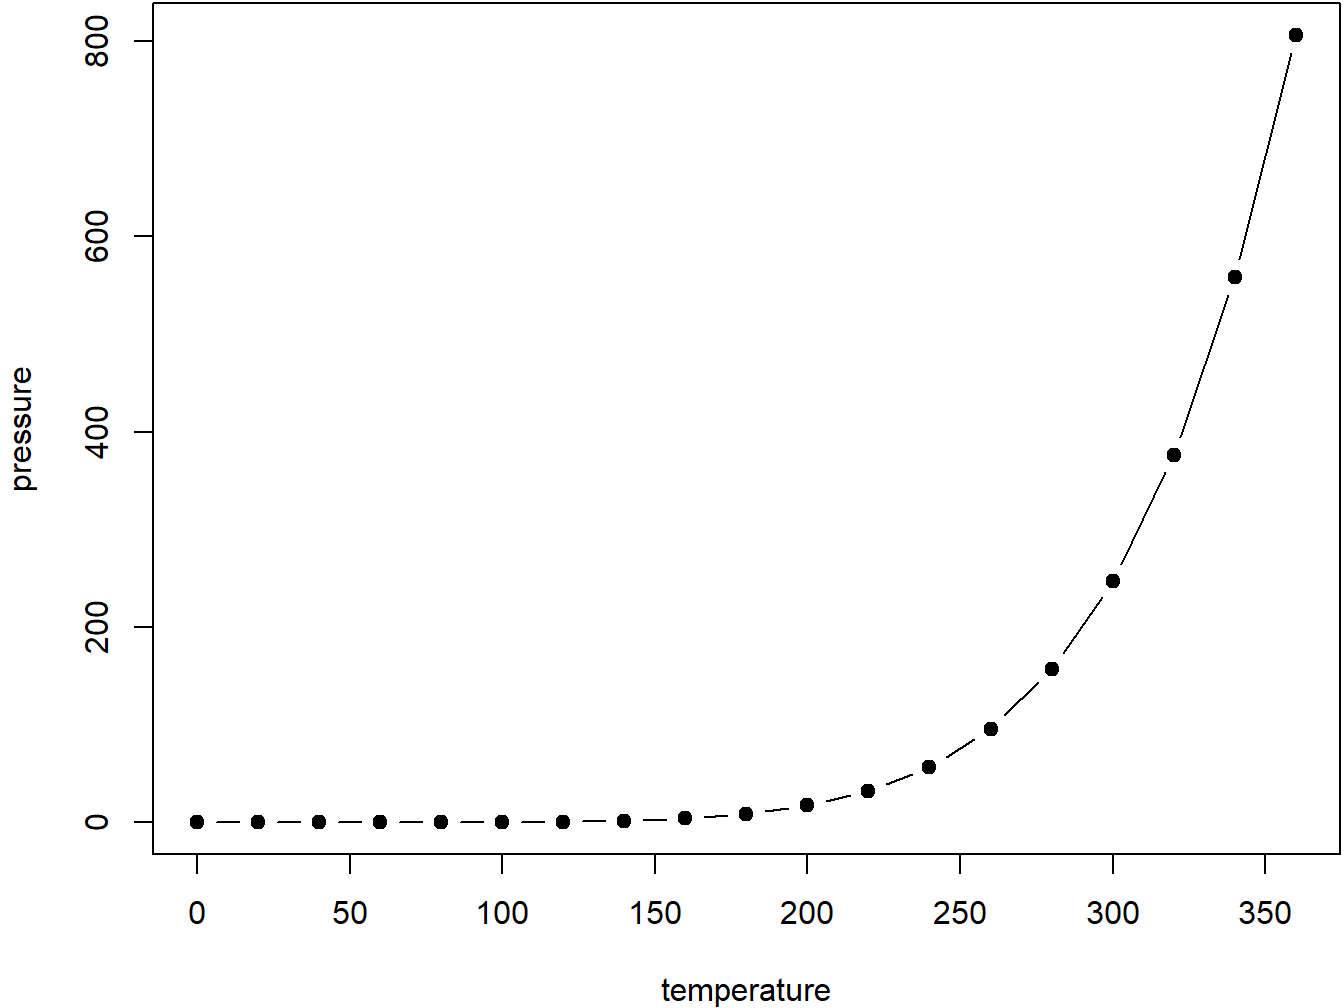
\includegraphics[width=0.8\linewidth]{R_Ref_Book_files/figure-latex/nice-fig-1} 

}

\caption{Here is a nice figure!}\label{fig:nice-fig}
\end{figure}

Reference a figure by its code chunk label with the \texttt{fig:}
prefix, e.g., see Figure \ref{fig:nice-fig}. Similarly, you can
reference tables generated from \texttt{knitr::kable()}, e.g., see Table
\ref{tab:nice-tab}.

\begin{Shaded}
\begin{Highlighting}[]
\NormalTok{knitr}\OperatorTok{::}\KeywordTok{kable}\NormalTok{(}
  \KeywordTok{head}\NormalTok{(iris, }\DecValTok{20}\NormalTok{), }\DataTypeTok{caption =} \StringTok{'Here is a nice table!'}\NormalTok{,}
  \DataTypeTok{booktabs =} \OtherTok{TRUE}
\NormalTok{)}
\end{Highlighting}
\end{Shaded}

\begin{table}

\caption{\label{tab:nice-tab}Here is a nice table!}
\centering
\begin{tabular}[t]{rrrrl}
\toprule
Sepal.Length & Sepal.Width & Petal.Length & Petal.Width & Species\\
\midrule
5.1 & 3.5 & 1.4 & 0.2 & setosa\\
4.9 & 3.0 & 1.4 & 0.2 & setosa\\
4.7 & 3.2 & 1.3 & 0.2 & setosa\\
4.6 & 3.1 & 1.5 & 0.2 & setosa\\
5.0 & 3.6 & 1.4 & 0.2 & setosa\\
\addlinespace
5.4 & 3.9 & 1.7 & 0.4 & setosa\\
4.6 & 3.4 & 1.4 & 0.3 & setosa\\
5.0 & 3.4 & 1.5 & 0.2 & setosa\\
4.4 & 2.9 & 1.4 & 0.2 & setosa\\
4.9 & 3.1 & 1.5 & 0.1 & setosa\\
\addlinespace
5.4 & 3.7 & 1.5 & 0.2 & setosa\\
4.8 & 3.4 & 1.6 & 0.2 & setosa\\
4.8 & 3.0 & 1.4 & 0.1 & setosa\\
4.3 & 3.0 & 1.1 & 0.1 & setosa\\
5.8 & 4.0 & 1.2 & 0.2 & setosa\\
\addlinespace
5.7 & 4.4 & 1.5 & 0.4 & setosa\\
5.4 & 3.9 & 1.3 & 0.4 & setosa\\
5.1 & 3.5 & 1.4 & 0.3 & setosa\\
5.7 & 3.8 & 1.7 & 0.3 & setosa\\
5.1 & 3.8 & 1.5 & 0.3 & setosa\\
\bottomrule
\end{tabular}
\end{table}

You can write citations, too. For example, we are using the
\textbf{bookdown} package \citep{R-bookdown} in this sample book, which
was built on top of R Markdown and \textbf{knitr} \citep{xie2015}.

\begin{center}\rule{0.5\linewidth}{\linethickness}\end{center}

We have finished a nice book.

\bibliography{book.bib,packages.bib}


\end{document}
